\let\negmedspace\undefined
\let\negthickspace\undefined
\documentclass[journal]{IEEEtran}
\usepackage[a5paper, margin=10mm, onecolumn]{geometry}
%\usepackage{lmodern} % Ensure lmodern is loaded for pdflatex
\usepackage{tfrupee} % Include tfrupee package

\setlength{\headheight}{1cm} % Set the height of the header box
\setlength{\headsep}{0mm}     % Set the distance between the header box and the top of the text

\usepackage{gvv-book}
\usepackage{gvv}
\usepackage{cite}
\usepackage{amsmath,amssymb,amsfonts,amsthm}
\usepackage{algorithmic}
\usepackage{graphicx}
\usepackage{textcomp}
\usepackage{xcolor}
\usepackage{txfonts}
\usepackage{listings}
\usepackage{enumitem}
\usepackage{mathtools}
\usepackage{gensymb}
\usepackage{comment}
\usepackage[breaklinks=true]{hyperref}
\usepackage{tkz-euclide} 
\usepackage{listings}
% \usepackage{gvv}                                        
\def\inputGnumericTable{}                                 
\usepackage[latin1]{inputenc}                                
\usepackage{color}                                            
\usepackage{array}                                            
\usepackage{longtable}                                       
\usepackage{calc}                                             
\usepackage{multirow}                                         
\usepackage{hhline}                                           
\usepackage{ifthen}                                           
\usepackage{lscape}
\begin{document}

\bibliographystyle{IEEEtran}

\title{5.2.26}
\author{EE25BTECH11023 - Venkata Sai}
% \maketitle
% \newpage
% \bigskip
\maketitle \vspace{-1cm}
\renewcommand{\thefigure}{\theenumi}
\renewcommand{\thetable}{\theenumi}
\setlength{\intextsep}{10pt} % Space between text and floats

\numberwithin{align}{enumi}
\numberwithin{figure}{enumi}
\renewcommand{\thetable}{\theenumi}

\textbf{Question:}  \\
Solve the following system of linear equations
\begin{align}
\frac{x}{a}-\frac{y}{b}=0 \\
ax+by=a^{2}+b^{2}
\end{align}

\textbf{Solution:}  
Given  
\begin{align}
\frac{x}{a}-\frac{y}{b}=0 \implies bx-ay=0 \\
ax+by=a^{2}+b^{2} 
\end{align}
The matrix equation for a line is defined as
\begin{align}
    \vec{n}^\top\vec{x}=c
\end{align}
where $\vec{n}$ is the coefficient matrix and $\vec{x}=\myvec{x\\y}$
\begin{align}
    \myvec{b&-a}\vec{x}=0
    \end{align}
    \begin{align}
    \myvec{a&b}\vec{x}=a^{2}+b^{2} 
\end{align}
As a matrix equation
\begin{align}
 \myvec{b&-a\\a&b}\vec{x}=\myvec{0\\a^{2}+b^{2}} 
  \end{align}
  \begin{align}
    \myvec{b&-a\\a&b}^\top\myvec{b&-a\\a&b}\vec{x}= \myvec{b&-a\\a&b}^\top\myvec{0\\a^{2}+b^{2}} 
    \end{align}
    \begin{align}
    \myvec{b&a\\-a&b}\myvec{b&-a\\a&b}\vec{x}= \myvec{b&a\\-a&b}\myvec{0\\a^{2}+b^{2}}  
  \end{align}
  \begin{align}
\myvec{a^{2}+b^{2}&0\\0&a^{2}+b^{2}}\vec{x}=\myvec{a\brak{a^{2}+b^{2}}\\b\brak{a^{2}+b^{2}}}
  \end{align}
  \begin{align}
\brak{a^{2}+b^{2}}\vec{I}\vec{x}=\myvec{a\brak{a^{2}+b^{2}}\\b\brak{a^{2}+b^{2}}} 
\end{align}
\begin{align}
\vec{I}\vec{x}=\myvec{a\brak{a^{2}+b^{2}}\\b\brak{a^{2}+b^{2}}} \frac{1}{a^{2}+b^{2}} 
  \end{align}
  \begin{align}
      \vec{I}\vec{x}=\myvec{a\\b}
  \end{align}
  \begin{align}
      \myvec{x\\y}=\myvec{a\\b}
  \end{align}
Hence $x=a,y=b$ is the solution for given system of linear equations
\begin{figure}[h!]
   \centering
   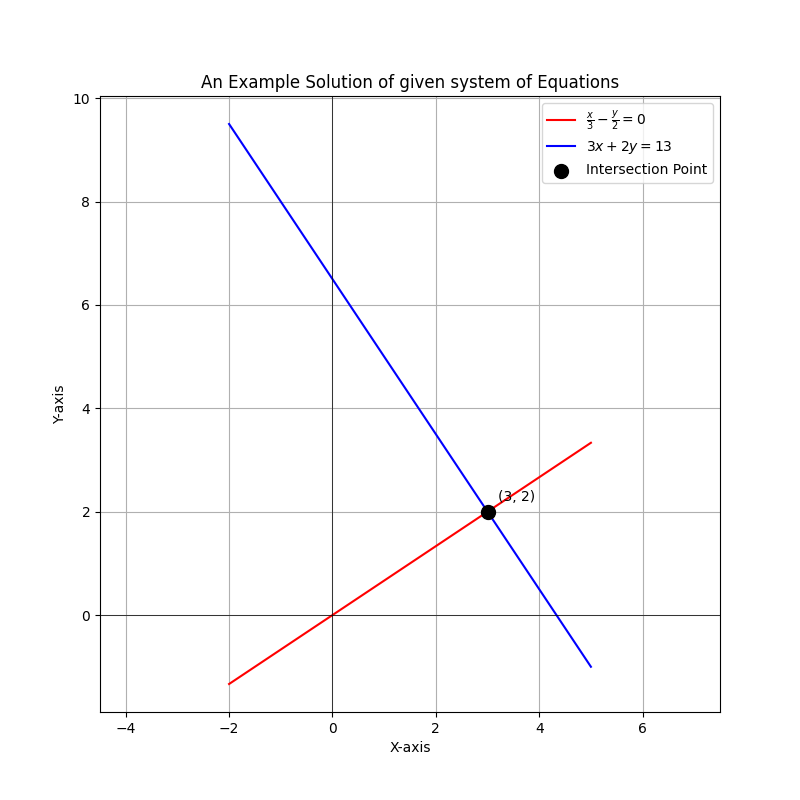
\includegraphics[width=0.7\columnwidth]{figs/fig1.png}
   \caption{}
   \label{Figure}
\end{figure}
\end{document}  